\chapter{Outer Detector Commissioning and Monitoring}\label{chap:ODCommissioning}
\section{OD PMT Calibration}
As discussed in \ref{sec:LZOD}, the primary purpose for the LZ Outer Detector is to detect neutron interactions which have coincident signals within the TPC. The source of most of the neutron background is from the ($\alpha$, n) process in material surrounding the edges of the xenon. A neutron will enter the TPC and then scatter out. The neutron can traverse the intervening material and then thermalize and capture on either the Gadolinium or the Hydrogen in the scintillator mixture or recoil off the protons in the scintillator. When the neutron recoils off the proton, energy depositions of $\sim$100~keV are produced \cite{LZNIMA}. The pulses of light detected in the PMTs for such low energy interactions are $\sim$15 photons in size and require the PMTs to be calibrated to a single photon sensitivity. Understanding the response of the PMTs is key to measuring single photon sensitivity and in turn reconstructing the gain of the PMTs. A model of photomultiplier response is presented in Ref.\cite{BELLAMY1994468} which will be described below.
\subsection{Single Photo-electron Response Model}\label{sec:SPhEResponse}
The PMT is considered to be an instrument which consists of two independent parts:
\begin{itemize}
    \item A photo-cathode where photons are converted into electrons
    \item An amplified which amplifies the initial charge (dynode system)
\end{itemize}
The model assumes that the number of photons incident on the PMT and subsequently the photo-cathode is a Poisson distributed variable. Only a fraction of the photons are converted to photo-electrons, this is the quantum efficiency of the PMT and is a random binary process ($\sim~25\%$ for the OD PMTs). The photo-electrons are then guided towards the first dynode by an electric field in which $\mathcal{O}(100\%)$ photo-electrons complete this process. The convolution of the Poisson and binary process results in a Poisson distribution:
\begin{equation}\label{eqn:SPEPoiss}
    P(n;\mu)=\frac{\mu^{n}e^{-\mu}}{n!},
\end{equation}
where $\mu$ is the mean number of photo-electrons collected at first dynode, $P(n;\mu)$ is the probability that $n$ photo-electrons are observed for a mean $\mu$.
The photo-electron is then amplified by the dynode system, which for the OD PMTs is a series of 10 dynodes. The amplification of the dynode system to determined by the voltage distribution across the dynode and it is tuned on a PMT-by-PMT basis to achieve a gain of $\mathcal{O}(10^6)$. The cascade of photo-electrons produced from the amplification is collected at the anode of the PMT and a voltage is measured as a pulse. The area of the pulse corresponds to number of electrons incident on the anode and is Gaussian distribution:
\begin{equation}\label{eqn:SPEGauss}
    G_n(x)=\frac{1}{\sigma_1\sqrt{2n\pi}}exp\biggl(-\frac{(x-nQ_1)^2}{2n\sigma_1^2}\biggl),
\end{equation}
where $x$ is the variable charge, $Q_1$ is the mean value of the charge outputted from the amplification at the dynode, $\sigma_1$ is the standard deviation of the charge amplification.
The ideal response an ideal PMT, $S_{ideal}$, can be described simply by convoluting \autoref{eqn:SPEPoiss} and \autoref{eqn:SPEGauss} together:
\begin{equation}
    \begin{split}
    S_{ideal}(x) & = P(n;\mu)\otimes G_n(x) \\
    & = \sum^\infty_{n=0}\frac{\mu^{n}e^{-\mu}}{n!}\frac{1}{\sigma_1\sqrt{2n\pi}}exp\biggl(-\frac{(x-nQ_1)^2}{2n\sigma_1^2}\biggl),
    \end{split}
    \label{eqn:PoisPlusGauss}
\end{equation}
the model is summed from 0 photons to an arbitrary upper limit \cite{BELLAMY1994468}.
\subsection{Single Photo-electron Calibration}
To calibrate the OD Single Photo-electron (SPhE) response, light is injected into the OD using the ODOCS. The optimal intensity of light to induce a SPhE response was chosen during the commissioning of the OD following the PMT installation in 2021. Details of the optimisation can be found in Ref.\cite{edfraser:thesis}.

Due to the complex geometry of the OD, the central row fibres were chosen as the injection points, position 2 in \autoref{fig:OCSPositions} (central row). Light injected from the central row fibres pass through the SATs and reflects back of the Tyvek\textregistered\ layer which covers the OCV.
Light injected from position 1 has the ability to pass direct through the TATs. Light injected from position 3 would be reflected within the BATs due to Tyvek\textregistered\ layers which was placed between the three acrylic tanks to cover foam which was needed to displace water. This later design decision was to increase light collection. Irregular gaps between BATs are present due to differences in moulding during construction of the BATs.

The OCS in configured so that 1000~photons are emitted from the end of the fibre. Due to attenuation of light in the fibre, 2000~photons must be emitted by the LEDs to account for a factor of two attenuation. For each injection of light, one of the 10 central row fibre emits 200,000~pulses at a 700~Hz injection rate. The rate of pulses injected was determined to not overload the LZ DAQ.

For ease of repeated measurement, an analysis module for the OD SPhE was developed to be used in conjunction with the LZ \textbf{P}hysics \textbf{RE}adiness \textbf{M}onitor (PREM) \cite{LZTDR}. The analysis module contains a selection to identify the OCS pulse and differentiate it from the background light seen in the OD. It be seen in \autoref{fig:ODSPhE_TimingSelection} that the OCS pulses are distributed around a peak at 560~ns after the trigger (which corresponds to 0~ns in \autoref{fig:ODSPhE_TimingSelection}). A selection of pulses with occurred between 500~ns and 700~ns after the DAQ was triggered by the OCS was chosen as an appropriate set of bounds for the timing selection to identify the OCS pulse. A PMT Coincidence requirement was also imposed to improve the purity of the selection as pulses with a coincidence greater than 1 PMT would likely not include any afterpulses which could mimic an OCS pulse.

\begin{figure}[ht!]
    \centering
    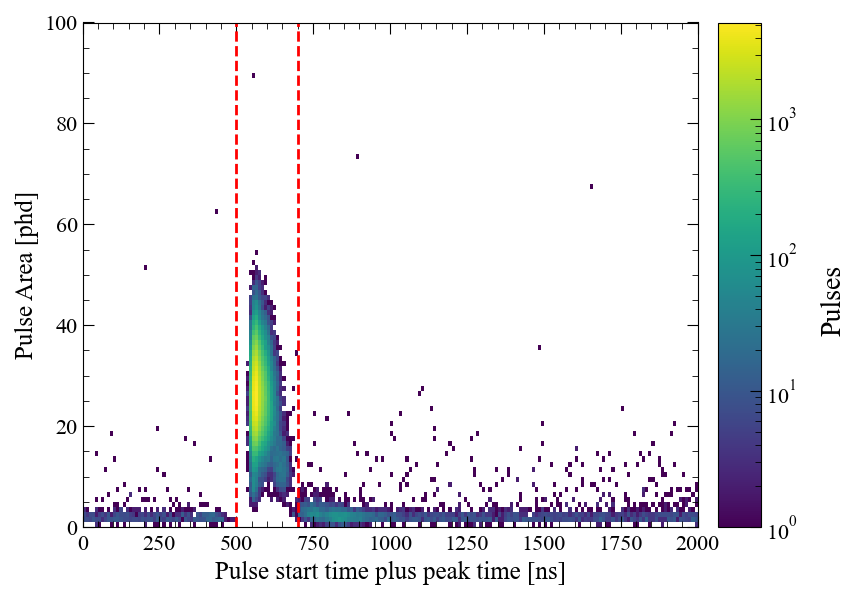
\includegraphics[width=0.8\linewidth]{figures/ODCommissioning/TimingVsPulseArea_2us.png}
    \caption{The response of the OD PMTs to 200k injections of 2000 photons during a monthly SPhE measurement. The pulse area is plotted against the start time of the pulse relative to the trigger plus the peak time relative to the start of the pulse. The OCS pulses are distributed around a peak of 560~ns. The two vertical dashed red lines indicate the inclusive timing selection criteria.}
    \label{fig:ODSPhE_TimingSelection}
\end{figure}

To measure the OD PMT's SPhE response \autoref{eqn:PoisPlusGauss} was used to fit the channel pulse area distributions. A two-stage fitting procedure was employed to account for the monthly variation in SPhE size across all 120 OD PMTs. The first stage of the procedure, only the single SPhE peak is fitted. Initially during commissioning, the starting value for $-\mu$ was determined by estimating the proportion of events in which no photon would be measured by the PMT. The mean and standard deviation (StD) of the histogram was used as starting values for components of the initial fit. The normalisation was taken to be the area beneath the curve between mean/4 and 6$\times$mean. The range in which to apply the fit was determined using the peak and defined from mean $\pm$ (Std/mean). In the second stage of the fitting procedure, the parameters from the initial fit were used as starting parameters to a fit of the multiple SPhE distribution. The range in which to apply the second stage fit was from mean - StD to mean + 3 StD. For each run only one fibre is used to inject light resulting in a small percentage of bad fits across the 120 PMTs depending on the particular fibre being used relative to the PMT of interest. To filter out such bad fits, only fits with $\chi^2/\text{ndf}<3$ were recorded for further analysis.

An example histogram and fit can be seen in \autoref{fig:ODSPhEDists}. It can be seen that the OD PMTs exhibit the expected response to SPhE as discussed in \autoref{sec:SPhEResponse}

\begin{figure}
     \centering
     \begin{subfigure}[b]{0.47\textwidth}
         \centering
         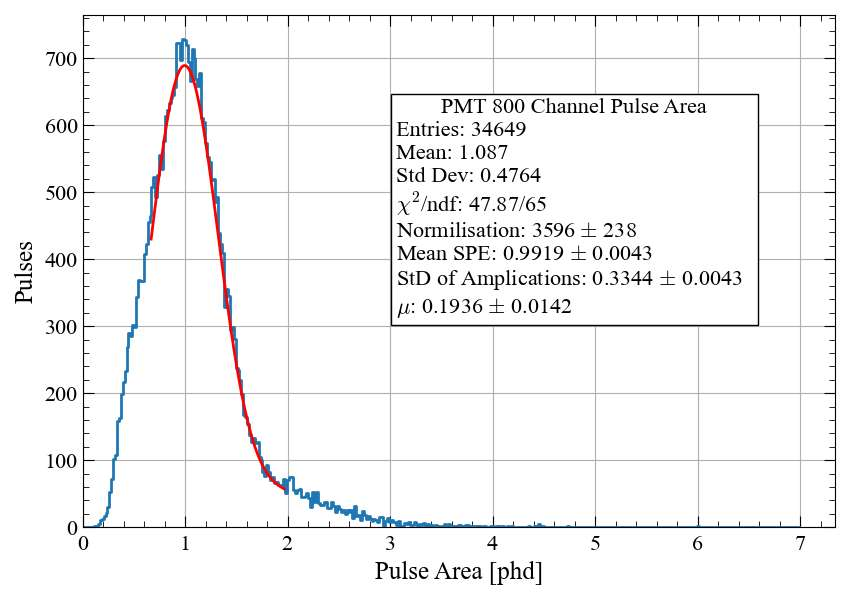
\includegraphics[width=\textwidth]{figures/ODCommissioning/PMT800_PulseArea_Distribution.png}
         \caption{}
         \label{fig:ODSPhE_phd}
     \end{subfigure}
%     \hfill
     \begin{subfigure}[b]{0.47\textwidth}
         \centering
         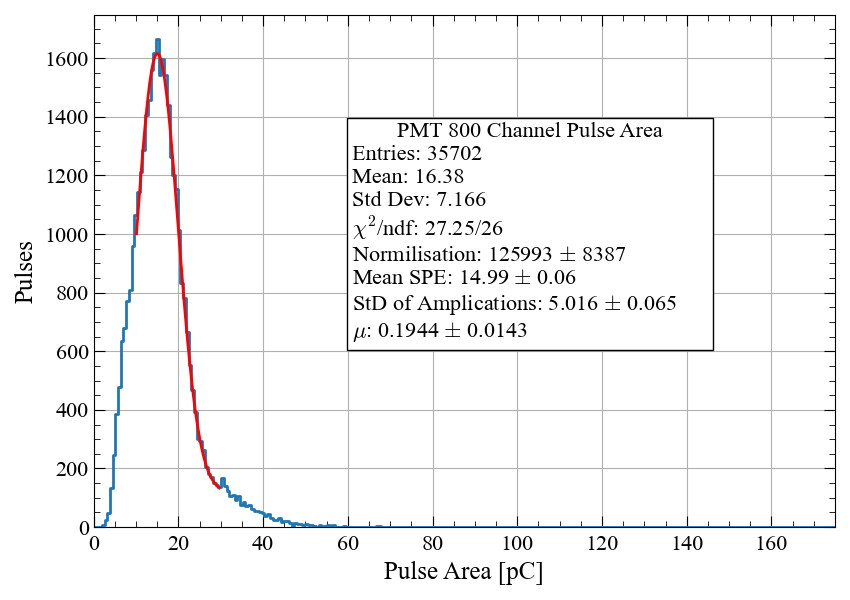
\includegraphics[width=\textwidth]{figures/ODCommissioning/PMT800_PulseArea_Distribution_pC.png}
         \caption{}
         \label{fig:ODSPhE_pC}
     \end{subfigure}
        \caption{Pulse area distributions of PMT 800 from 200k OCS injections of 2000 photons during OD SPhE measurement. \textbf{Left:} Reconstructed pulse area measured in photons detected. \textbf{Right:} Pulse area taken from the area measured in the raw waveform in mVns, and converted to pC by dividing by the $50~\Omega$ termination at the amplifier. The fit applied in red is \autoref{eqn:PoisPlusGauss} and the constants can be seen in the respective statistics boxes on each plot.}
        \label{fig:ODSPhEDists}
\end{figure}
An example PMT calibration is outlined below for PMT 800. The mean Gaussian response is (0.9919 $\pm$ 0.0043) phd and (14.99 $\pm$ 0.06) pC. The SPhE calibration constant used to process the raw data is reconstructed by dividing the SPhE response measured in mVns by the SPhE response measured in phd, which in this case for PMT 800 is 753.9~mVns. These three values together are stored in the PREM database. In a secondary analysis stage, the measured SPhE area and calibration constant are combined to get the correct SPhE constant in mVns which in this example is 748.5~mVns. The average is taken of the corrected SPhE constant for all 10 measurements corresponding to the 10 central row OCS fibre injections. The new SPhE constant is then transferred to the LZ Conditions database along with the data and time period for which this constant is valid for. As LZ then continues to collect data, the raw pulse area measured in mVns is converted to phd by dividing the raw area by the constant. Examples of the variation in measured SPhE in both phd and mVns across all 120 PMTs is shown in \autoref{fig:SPhEValues_phd} and \autoref{fig:SPhEValues_pC}.
\begin{sidewaysfigure}[ht!]
    \centering
    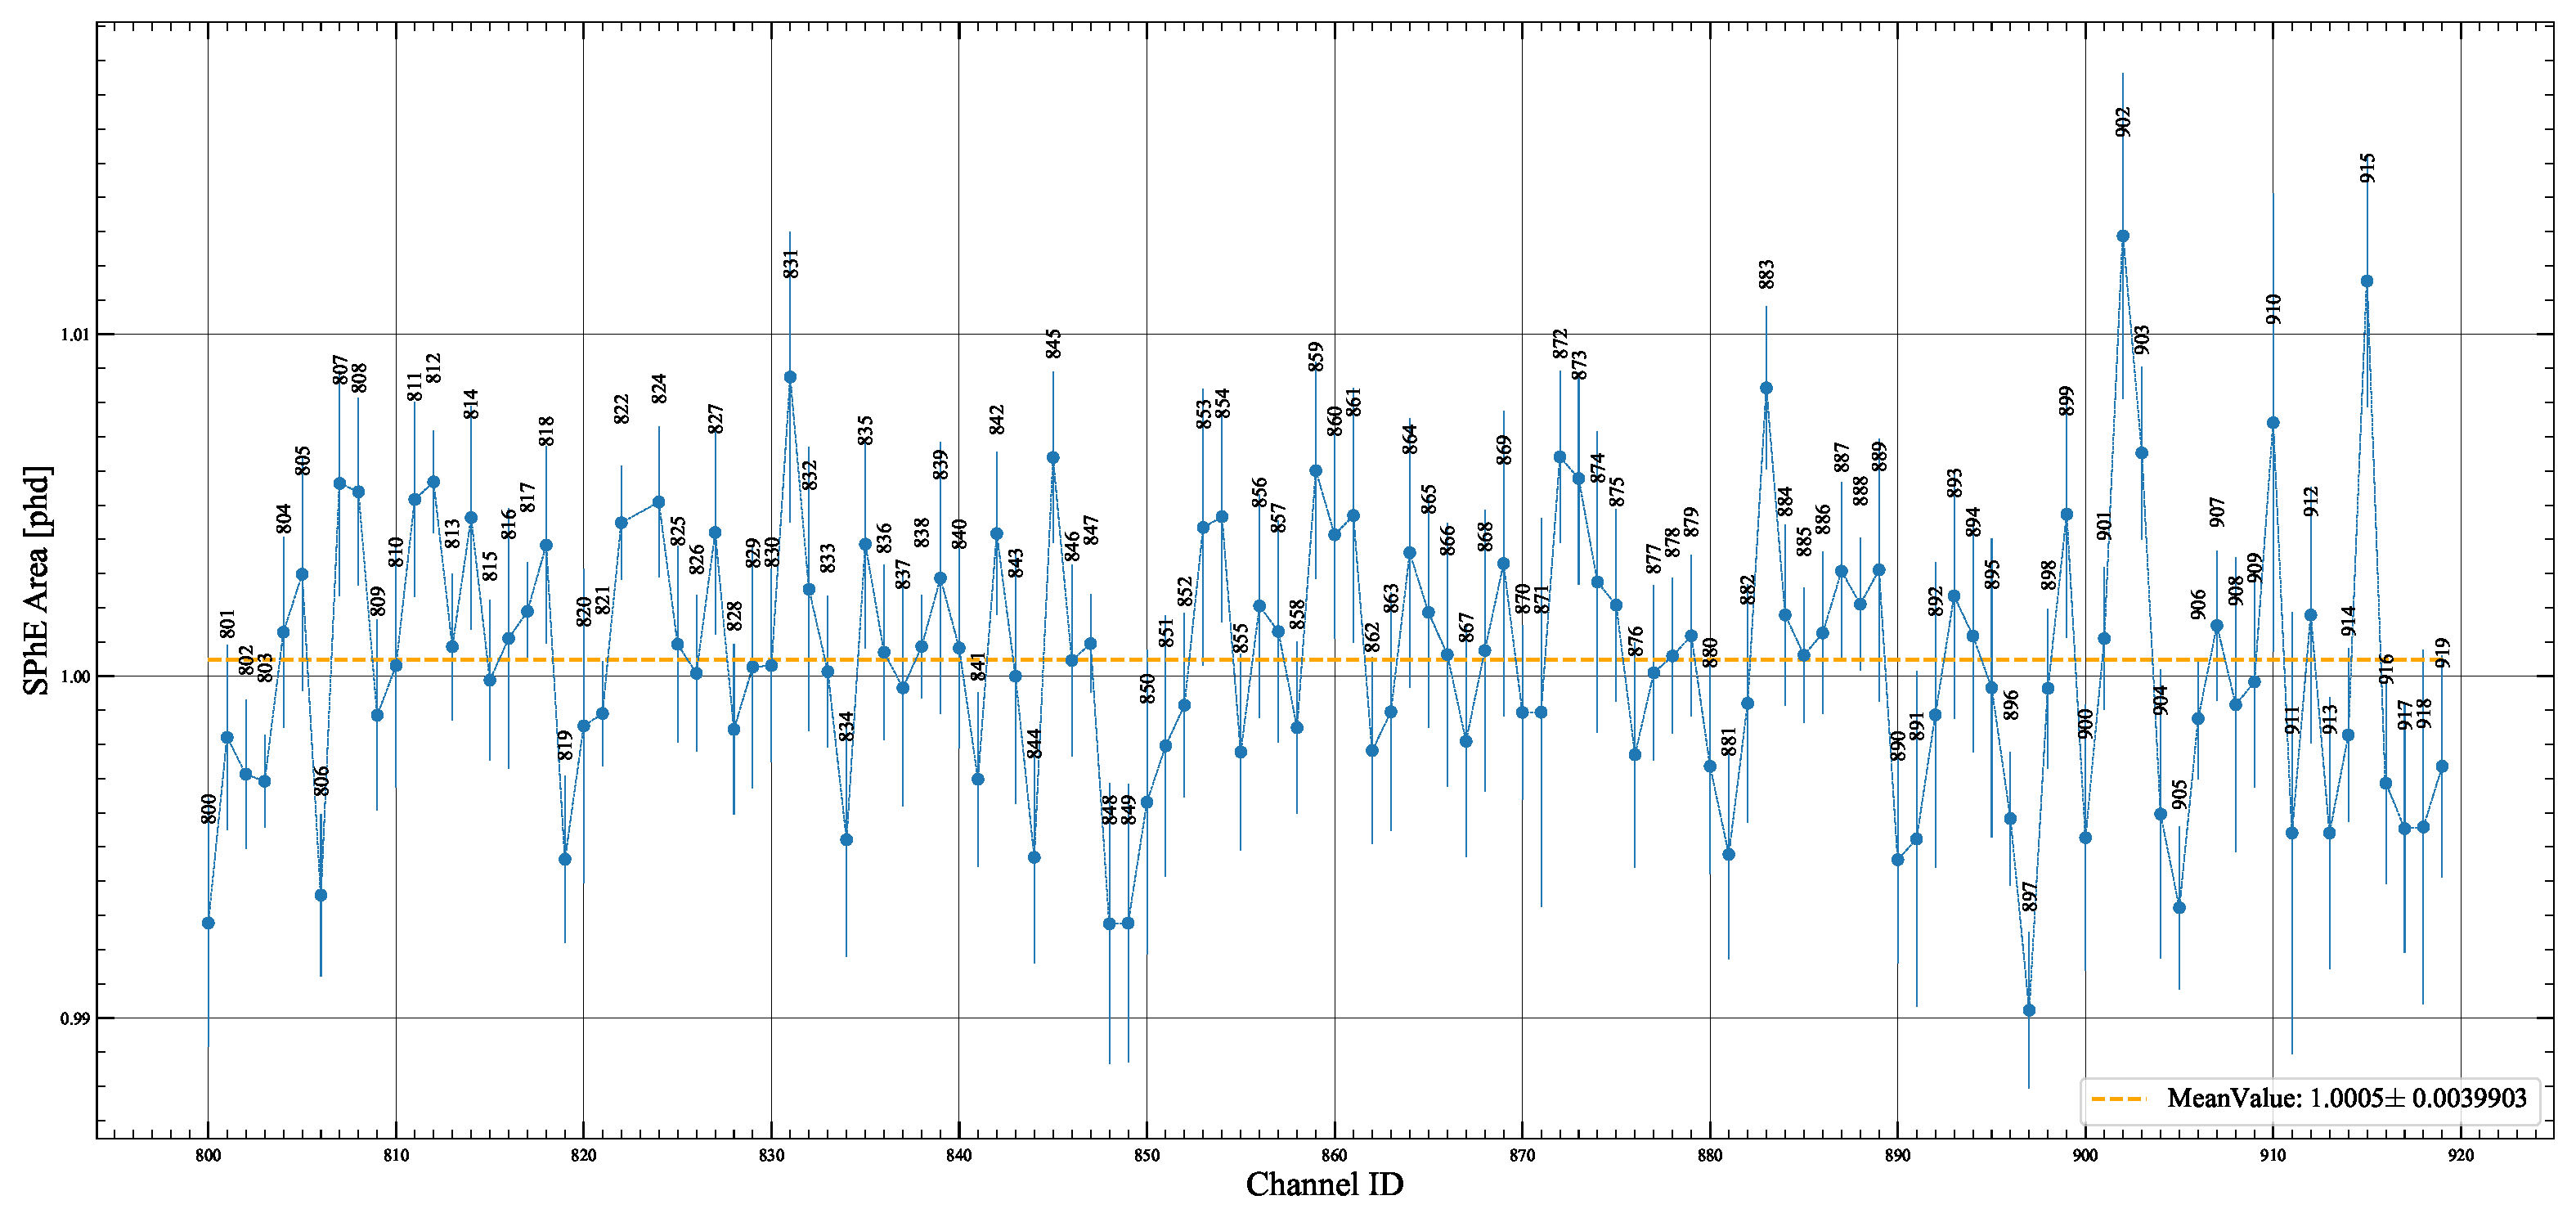
\includegraphics[width=\textwidth]{figures/ODCommissioning/SPHE_phd_2025-2-12.pdf}
    \caption{A scatter plot of the OD SPhE Area size measured in phd versus Channel ID for each OD PMT from a measurement taken on February 12th 2025.}
    \label{fig:SPhEValues_phd}
\end{sidewaysfigure}
\begin{sidewaysfigure}[ht!]
    \centering
    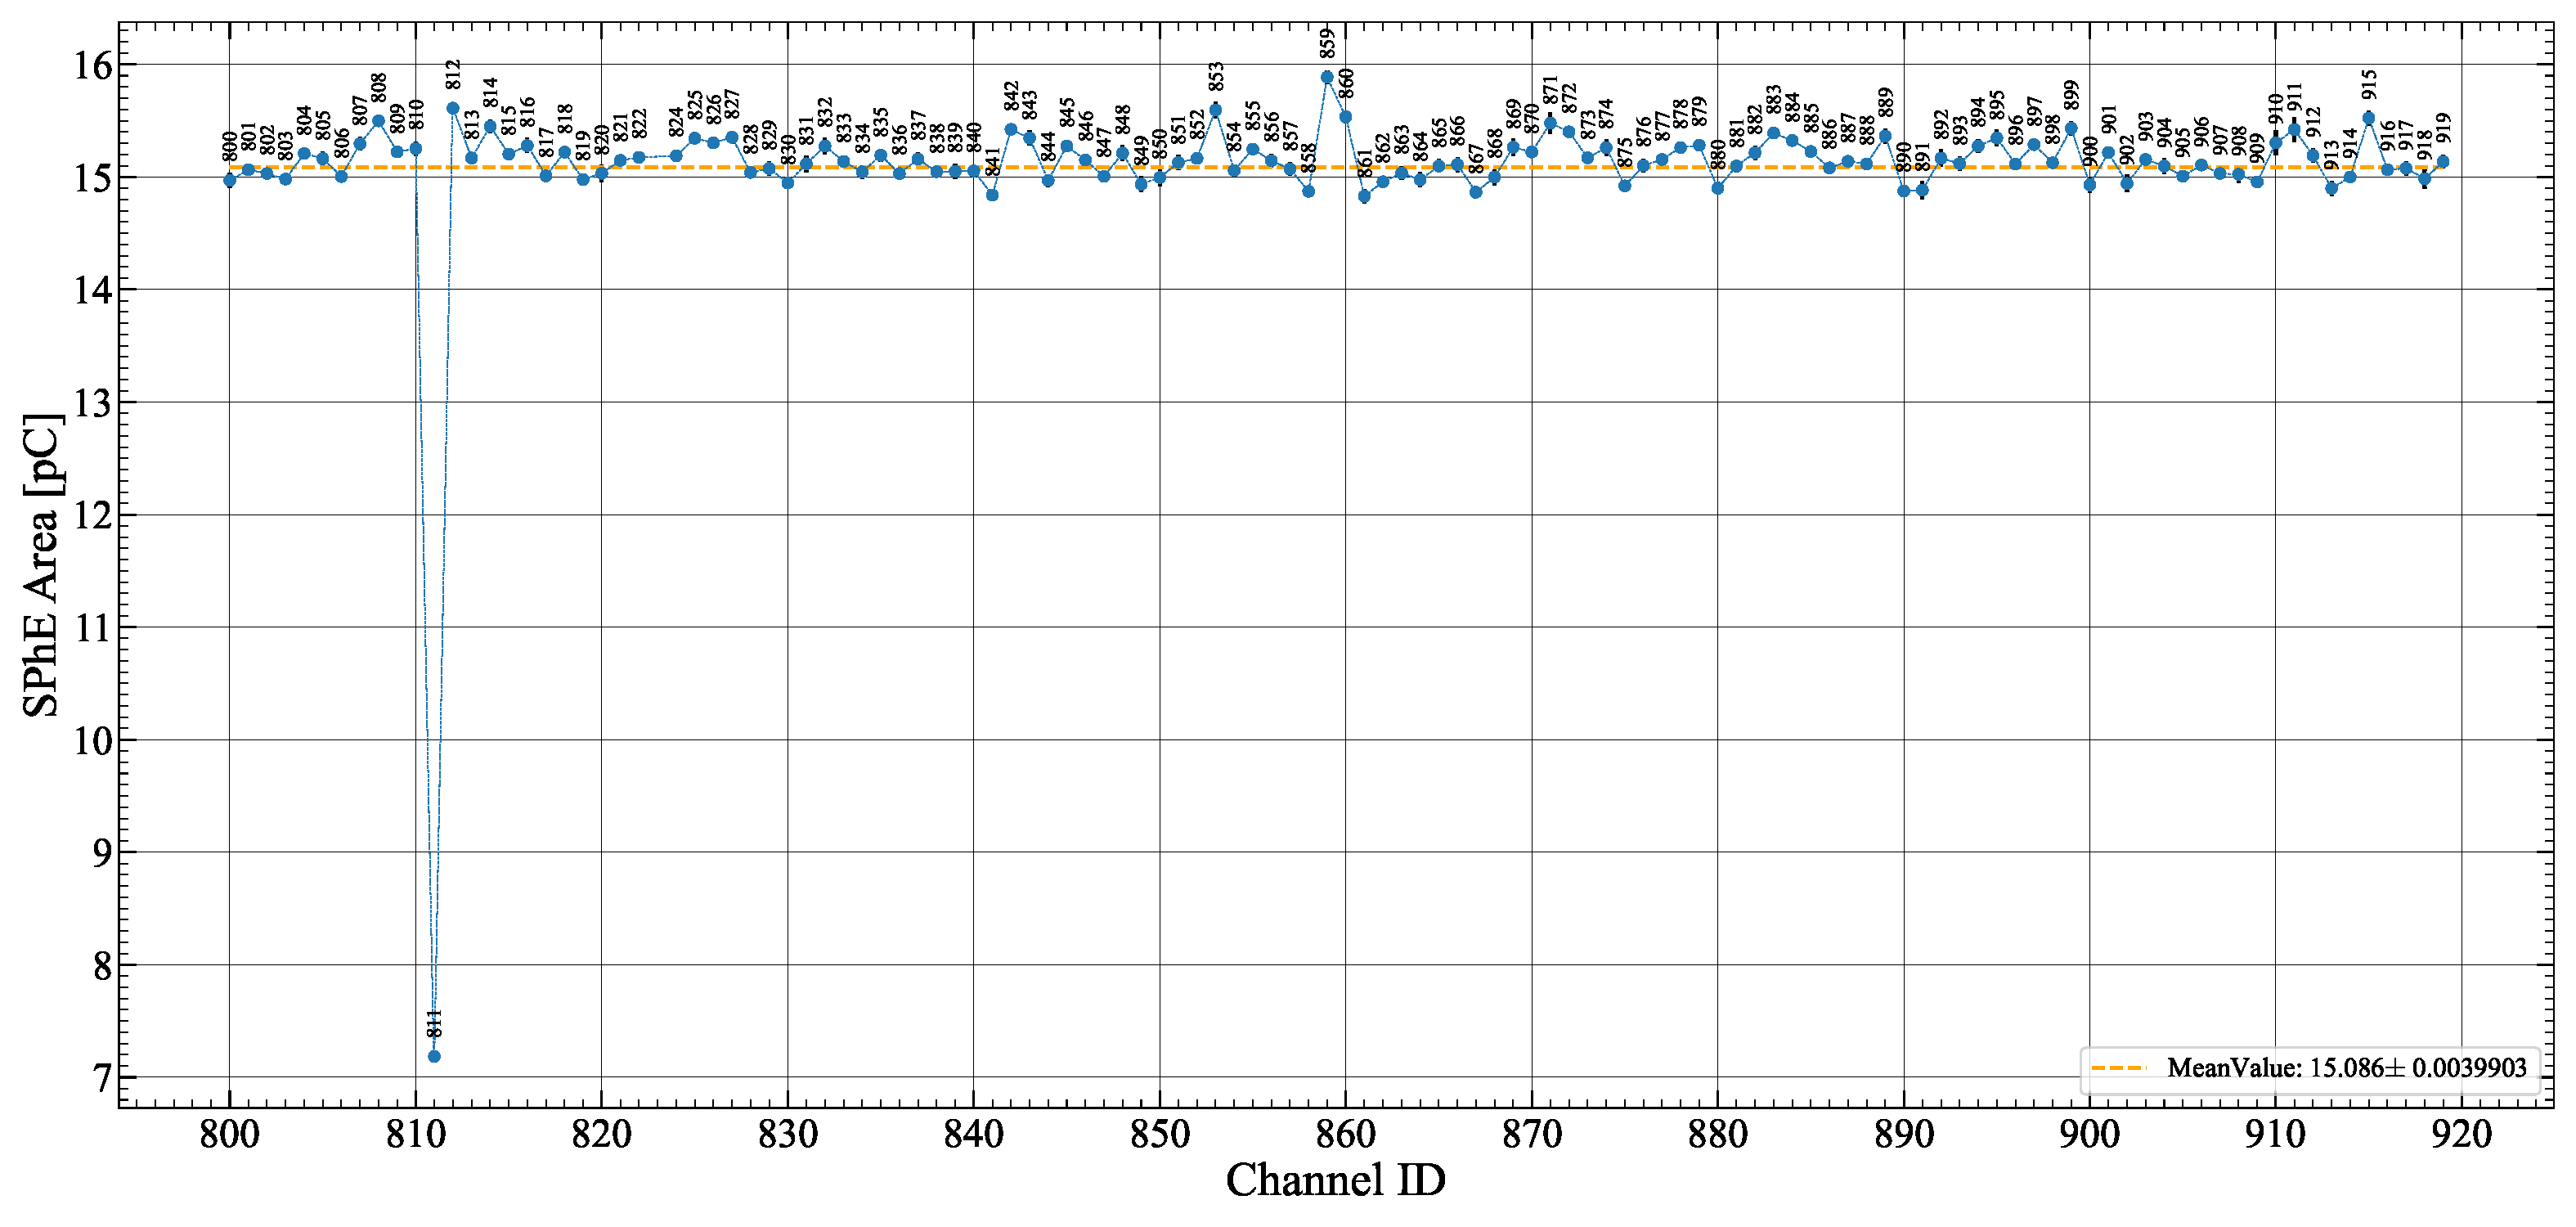
\includegraphics[width=\textwidth]{figures/ODCommissioning/SPHE_pC_2025-2-12.pdf}
    \caption{A scatter plot of the OD SPhE Area size measured in mVns versus Channel ID for each OD PMT from a measurement taken on February 12th 2025.}
    \label{fig:SPhEValues_pC}
\end{sidewaysfigure}
\section{Reconstructed Gain}
So far it has been shown that understanding how the signal from a PMT relates to the amount of light incident on the face of the PMT. The amplification of the photoelectrons produced through the cascade through the dynode series is known as the PMT's `Gain'. The SPhE Calibration Constant can be converted to gain by dividing by the following terms, $e\times44\times10^{12}$, where 44 is the amplification factor in the amplifier, e is the charge of an electron, $10^{12}$ accounts for the change with the unit prefixes on voltage and time. As this 

\subsection{Gain Curves}
\subsection{Monitoring PMT Health Over Time}

\section{Trigger Efficiency}

\section{Optical Calibration System Development}
\subsection{UV LED commissioning}

\subsection{Monitoring PMT}